\documentclass{article}
% TITLE PAGE CONTENT %%%%%%%%%%%%%%%%%%%%%%%%
% Remember to fill this section out for each
% lab write-up.
%%%%%%%%%%%%%%%%%%%%%%%%%%%%%%%%%%%%%%%%%%%%%
\usepackage{CJK}
\usepackage{float}
\usepackage{subfig}
\usepackage{graphicx}
\usepackage{listings} % For source cod
\usepackage{xcolor}
\usepackage{geometry}
\geometry{left=1.7cm,right=1.7cm,top=2.0cm,bottom=2.0cm}
\usepackage{float}
\usepackage{subfig}
% END TITLE PAGE CONTENT %%%%%%%%%%%%%%%%%%%%


\begin{document}  % START THE DOCUMENT!

\begin{CJK}{UTF8}{gkai}
\title{实验五 单片机串行通信}
\author{杨庆龙 \\1500012956}
\date{2018.4.18}
\maketitle
\section{实验目的}
\begin{itemize}
  \item 了解串行通信的基本知识
  \item 掌握用单片机串行口实现串行通信的方法
\end{itemize}
\section{实验原理}
\subsection{串行通信的异步和同步传送方式}
CPU与外设的基本通信方式可分为并行通信和串行通信两类。并行是指要传输的的按照二进制位同时传输,串行则是逐位传输的方式。\\
串行传输所用的传输线远少于并行传输线,也是实际常用的传输线。\\
单片机使用异步传输的通信方式,其特点为
\begin{itemize}
  \item 数据是离散发送的
  \item 通信双方时钟频率相同
  \item 通信双方按照异步通信协议传输字符
\end{itemize}
字符帧格式为,一个起始位,N位数据位,一个校验位,一个停止位\\
异步通信使用波特率=单帧位数*每秒的帧数表示数据传输的速率。并使用高于传输速率的时钟进行采样提高采样的准确性。
\subsection{MCS-51的串行通信接口}
MCS51内部有一个可编程的全双工串行通信口,可作为通用异步接收和发送器,也可作为同步移位寄存器使用。内部的串行通信口,有两个独立的接收发送缓冲器SBUF,对外也有两条独立的收发信号线RxD和TxD。可以同时发送,接收数据,实现全双工传送。与串行通信有关的寄存器有多个,用SCON控制和监视串行口的工作状态。
\begin{table}
  \centering
  \caption{串行控制寄存器SCON}
  \begin{tabular}{|c|c|c|c|c|c|c|c|}
    \hline
    D7&D6&D5&D4&D3&D2&D1&D0\\
    \hline
    SM0&SM1&SM2&REN&TB8&RB8&TI&RI\\
    \hline
  \end{tabular}
\end{table}
\begin{itemize}
  \item SM0,SM1:00,同步移位寄存器,01,8位UART,10,9位UART,11,9位UART可变波特率
  \item REN:允许接收控制位,由软件置位或清除
  \item TB8:模式2,33中的第九位
  \item RB8:该位是模式2和3中已接收的第九位
  \item TI:发送中断标识
  \item RI:接收中断标识
\end{itemize}
\section{实验内容}
\subsection{观察UART通信波形}
设定串行口工作方式1,用1200bps循环发送一个字节55H或8AH,用示波器观察TxD的电平和信号结构,给出1200bps波特率条件下的TH1计算值,码元宽度的计算值和测量值。
\subsection{串口收发实验}
编写一个程序是单片机通过键盘输入数据,再把数据送到PC上,PC又将数据发送给单片机,单片机将数据现实到数码管上。
\subsection{串口作为STDIO}
初始化了UART0后,单片机会将该串口作为STDIO,用户可以直接用printf和scanf从串口中读写数据。编写程序通过串口输入数据,进行四则运算后输出到串口。
\section{实验结果}
\subsection{观察UART通信波形}
<<<<<<< HEAD
设定串口工作方式1,用9600bps的波特率,发送8AH,用示波器观察TxD可得\ref{pro1_1}。从图中可以看到,串口输出信号为0010100011,输出波形符合预期,接下来是波特率检查。
\begin{figure}
  \centering
  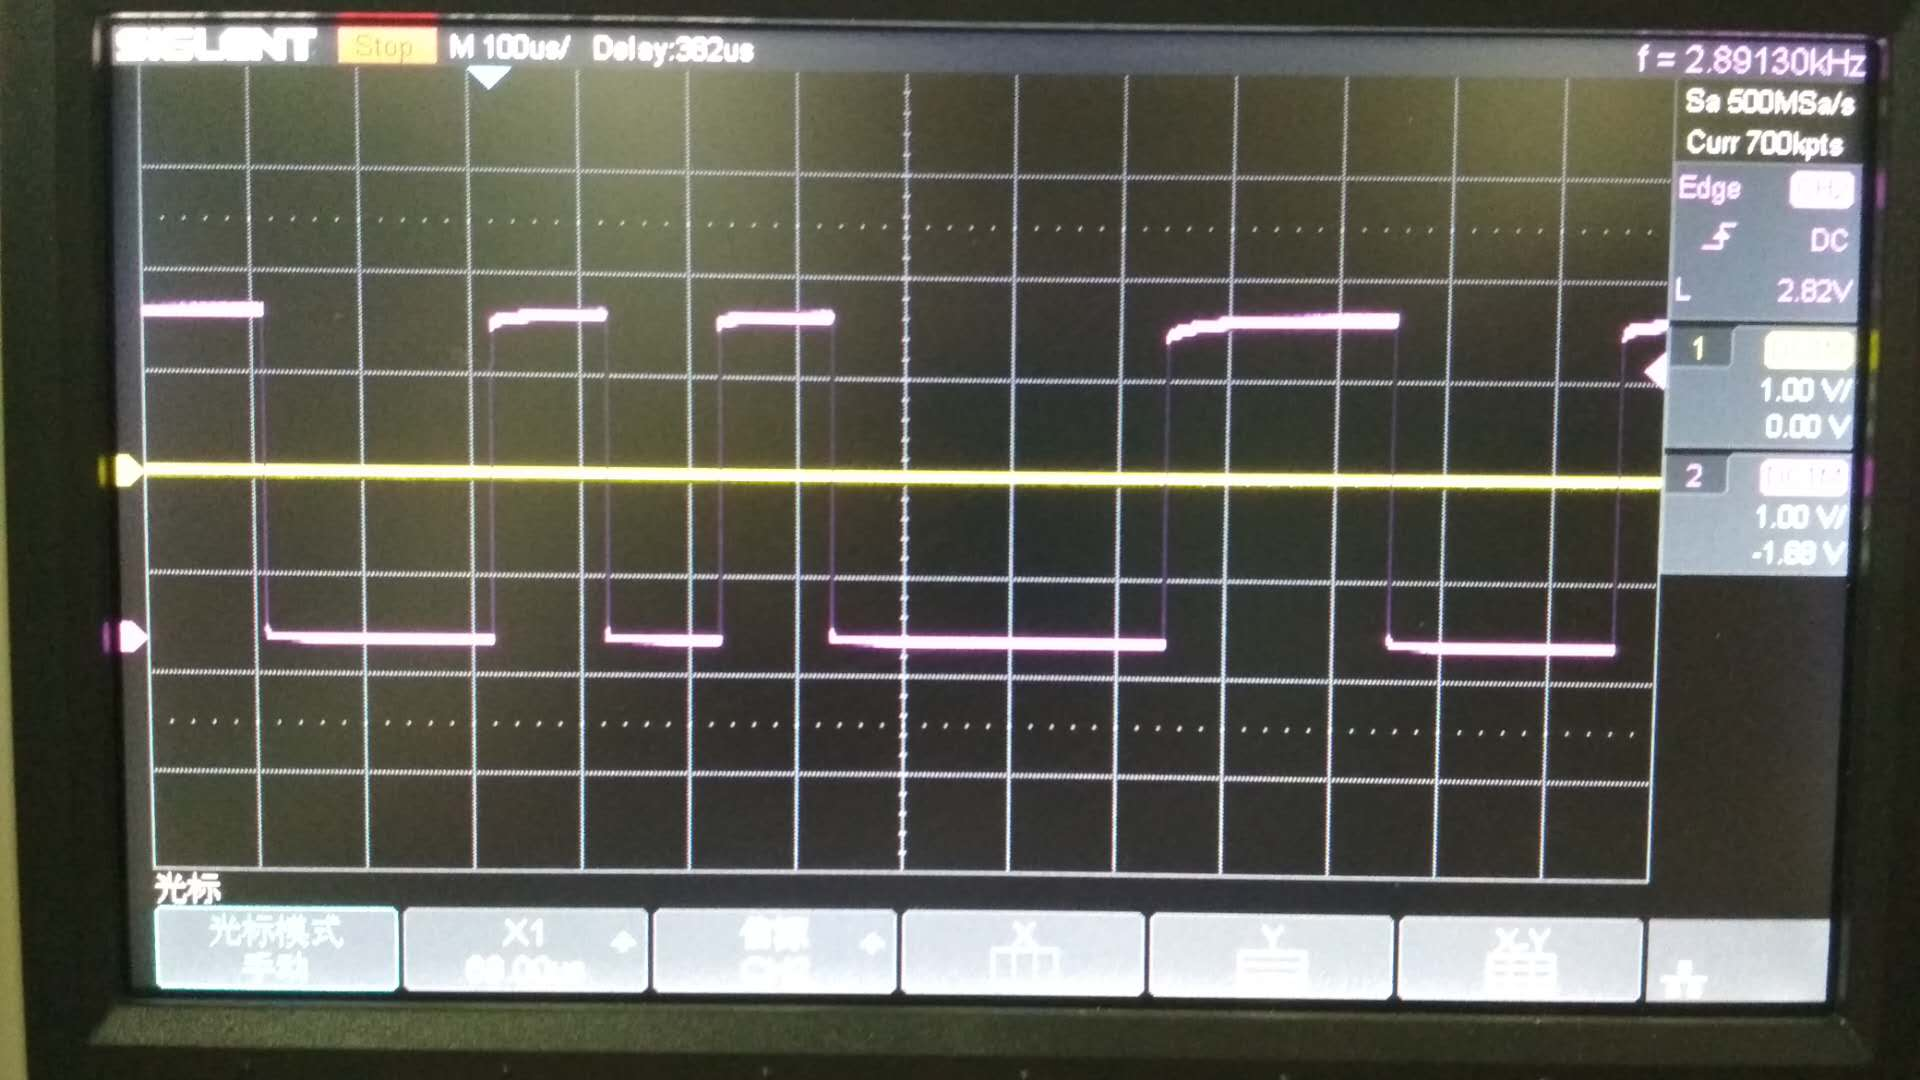
\includegraphics[width=0.6\textwidth]{code.jpg}
  \caption{8AH信号波形}
  \label{pro1_1}
\end{figure}
设置保持串口工作方式不变,波特率不变,输出55H,用示波器观察TxD可得图像如\ref{pro1_2},使用示波器的measure功能测量得到,信号频率为4.8kHz的方波,即为9600bps的信号波形。
\begin{figure}
  \centering
  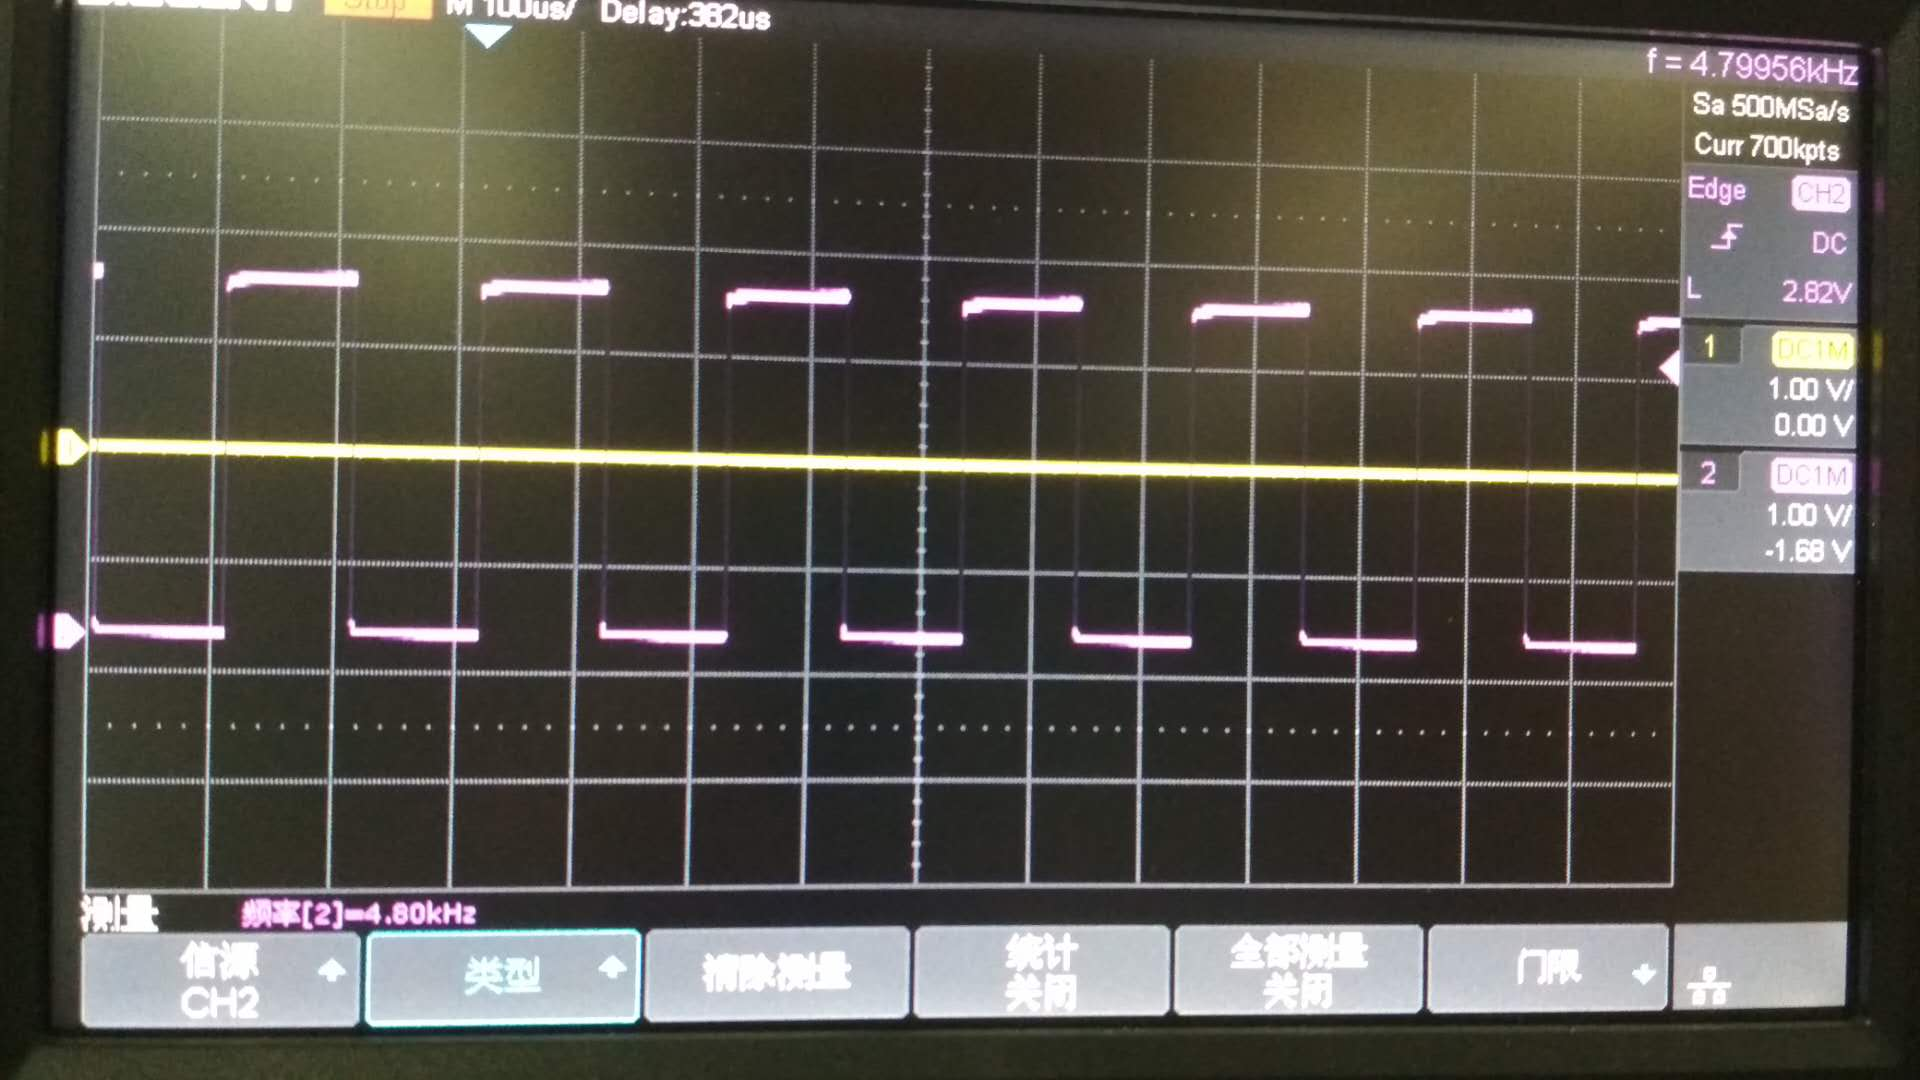
\includegraphics[width=0.6\textwidth]{frequency.jpg}
  \caption{55H信号波形}
  \label{pro1_2}
\end{figure}
\subsection{串口收发实验}
按动按键,可以在PC机的串口监视器上看到相应的按键,使用串口监视器向开发板发送0到9的数字,可以在开发板的发光数码管上显示相应的数字,满足设计要求。
\begin{figure}
  \centering
  \subfloat[发送端截图]{\label{pro2_1}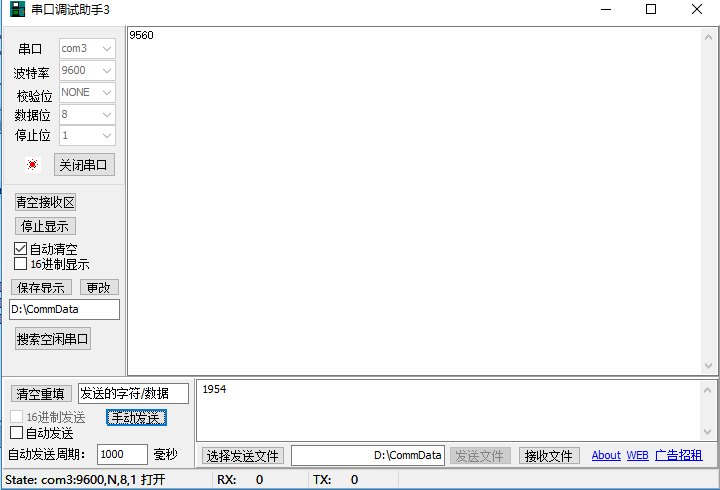
\includegraphics[width=0.4\textwidth]{read.png}}
  \subfloat[数码管显示]{\label{pro2_2}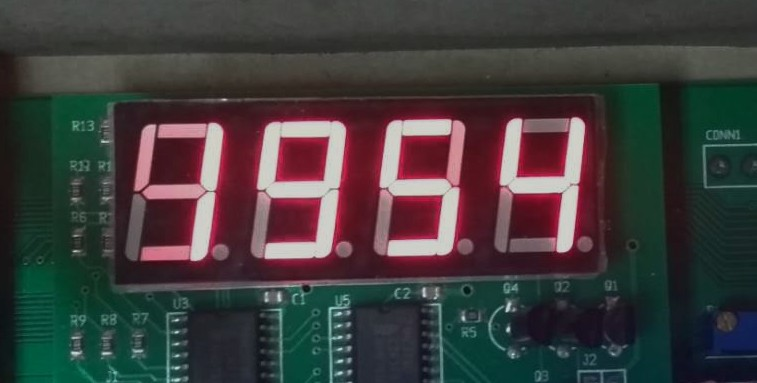
\includegraphics[width=0.4\textwidth]{display.jpg}}
  \caption{串口通信实验结果图}
\end{figure}
\subsection{串口作为STDIO}
从串口读入两个操作数和操作符,并将计算结果输出到串口上,结果如图\ref{pro3_1}。
\begin{figure}
  \centering
  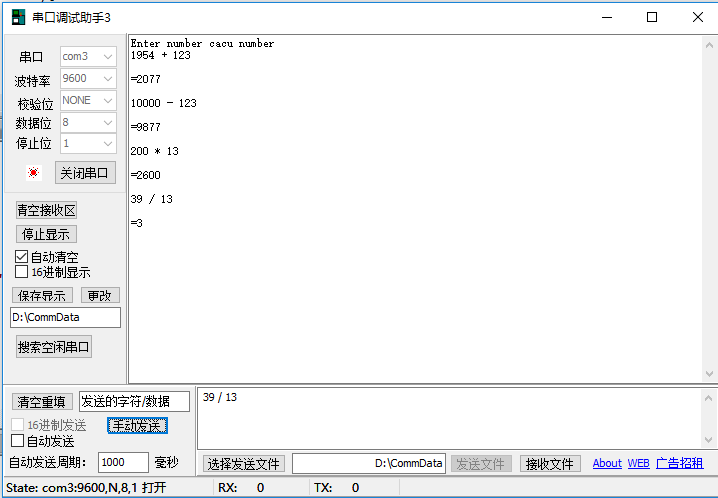
\includegraphics[width=0.6\textwidth]{cacu.png}
  \caption{计算结果}
  \label{pro3_1}
\end{figure}
\section{思考题}
\begin{enumerate}
  \item 例如,当接收方时钟为发射方两倍时,发射方每发出一个bit,接收方都会收到两个同样的bit,这就会导致接收方收到的数据有误。
  \item 使用系统时钟对230400bps分频,再依据采样率计算得到计数器溢出数字即可。例如对于 16倍采样率有22118400/230400/16=6。对于300bps可以得到相同的结论,计数器赋值为22118400/300/16=4608.
\end{enumerate}
\section{源码}
\subsection{观察UART通信波形}
\begin{lstlisting}[language=C,numbers=left,numberstyle=\tiny,%frame=shadowbox,
   rulesepcolor=\color{red!20!green!20!blue!20},
   keywordstyle=\color{blue!70!black},
   commentstyle=\color{blue!90!},
   basicstyle=\ttfamily]
#include <C8051F020.h>
#include "../../includes/time.h"
#include "../../includes/communicate.h"
void main() {
  WDTCN = 0xDE;
  WDTCN = 0xAD;
  sysclk_init();
  uart0_port_init();
  uart0_init();
  while (1) {
    SBUF0 = 0x55;//0x8A
    while(!TI0);
    TI0 = 0;
  }
}

\end{lstlisting}

\subsection{串口收发实验}
\begin{lstlisting}[language=C,numbers=left,numberstyle=\tiny,%frame=shadowbox,
   rulesepcolor=\color{red!20!green!20!blue!20},
   keywordstyle=\color{blue!70!black},
   commentstyle=\color{blue!90!},
   basicstyle=\ttfamily]
   #include <C8051F020.h>
   #include "../../includes/communicate.h"
   #include "../../includes/keyboard.h"
   #include "../../includes/display.h"
   #include "../../includes/storage.h"
   #define RX_LEN 4
   #define EMPTY 255
=======
设定串口工作方式为1,实际所用波特率为9600,传输字节为8AH。用示波器观察TxD的电平,得到波形图如下。
\begin{figure}
  \includegraphics[width=0.5\textwidth]{pro1_sub1.jpg}
  \caption{9600波特率8AH波形图}
  \label{pro1_sub1.jpg}
\end{figure}
\subsection{串口收发实验}
\begin{figure}
  \includegraphics{pro2_sub1.jpg}
  \caption{}
  \label{pro2_sub2.jpg}
\end{figure}
\subsection{串口STDIO}
>>>>>>> 39c049beb19b1056eb1ee906be3afdf5f37b94bf

   int RxBuf[RX_LEN];
   char TxBuf;
   uchar keyResult;

   void main() {
     WDTCN = 0xDE;
     WDTCN = 0xAD;
     sysclk_init();
     uart0_port_init();
     uart0_init();
     storage_port_init();
     int0_init(SYSCLK / 800);
     ES0 = 1;
     EA = 1;
     TxBuf = '\0';
     while(1) {
     	delay(1000);
       keyResult = getKey();
       if(keyResult != NOKEY) {
   	    SBUF0 = keyResult + '0';
   		keyResult = NOKEY;
   		TI0 =1;
   	}
     }
   }

   void uart0_int() interrupt 4 {
     char c;
     if(RI0 == 1) {
       RI0 = 0;
       c = SBUF0;
   	c -= '0';
       RxBuf[3] = RxBuf[2];
       RxBuf[2] = RxBuf[1];
       RxBuf[1] = RxBuf[0];
       RxBuf[0] = c;
     }
     else if(TI0 == 1)
     TI0 = 0;
   }

   void time0_int() interrupt 1 {
     static int index = 0;
     index ++;
     index %= 4;
     digital_selecte = digital_index[index];
     if(RxBuf[index] < 16)
       digital_number = digital_trans[RxBuf[index]];
     else
       digital_number = digital_trans[16];
   }

\end{lstlisting}
\subsection{串口作为STDIO}
\begin{lstlisting}[language=C,numbers=left,numberstyle=\tiny,%frame=shadowbox,
   rulesepcolor=\color{red!20!green!20!blue!20},
   keywordstyle=\color{blue!70!black},
   commentstyle=\color{blue!90!},
   basicstyle=\ttfamily]
   #include <C8051F020.h>
   #include <stdio.h>
   #include "../../includes/communicate.h"
   #include "../../includes/time.h"

   int main() {
     int a,c,result;
     char b;
     WDTCN = 0xDE;
     WDTCN = 0xAD;
     sysclk_init();
     uart0_port_init();
     uart0_init();
     TI0 = 1;
     printf("Enter number cacu number\n");
     while(1) {
       if(scanf("%d %c %d",&a,&b,&c)) {
         switch(b) {
           case '+' :
   		result = a+c;
           break;
           case '-':
   		result = a-c;
           break;
           case '*':
   		result = a*c;
           break;
           case '/':
   		result = a/c;
           break;
   		default:
   		result = -1;
         }
   	  printf("\r\n=%d \r\n",result);
       }
     }
   }

\end{lstlisting}
\end{CJK}
\end{document} % DONE WITH DOCUMENT!


\\
学校里,提供二维码,为需要物品打标签。
钥匙打码
可选打码
